%Only use subsection and subsubsection
\subsection{Motivation}

Traditionally, complex interfaces are used to command robots (joystick, remote, steering wheel, etc). The main goal is to create an easy interface for an untrained operator using natural linguistic language. The robot needs to learn movement that was shown by the operator, and then process it in order to learn from a demonstration. For this reason, the work is based on an incremental learning from a demonstration delivered by a kinesthetic correction.

The operator will shows the robot how to move to an order by doing a kinesthetic demonstration.\\

\begin{figure}[H]
\centering
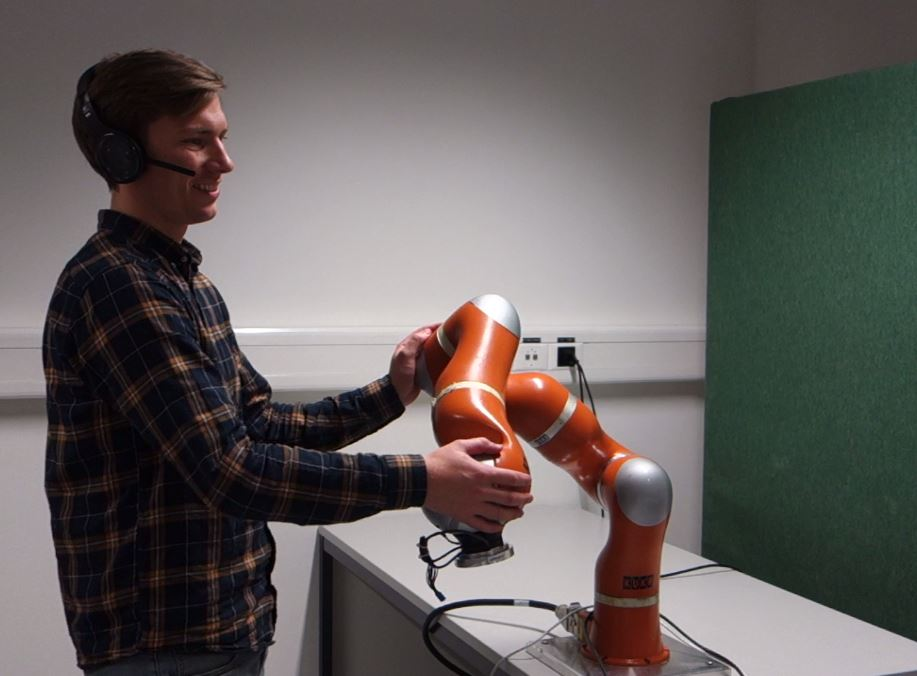
\includegraphics[width=10cm]{img/klas_dem.jpg}
\caption{An operator doing a kinesthetic demonstration.}
\end{figure}

On this project, we worked on the demonstration processing, how the robot understands the movement that was shown to it.

\subsection{Background} 

This project is an incremental work, the robot already knows how to move from one point to another. To show to the robot how to move, the operator needs to do a kinesthetic demonstration. To do so, a target point (or attractor point) is numerically set somewhere reachable in the space and the robot will move to this point. The mission of the operator will be to shift the robot from its trajectory by taking it with his own hands and applying a kinesthetic correction on it. This is a correction on the trajectory, it will be a movement that the robot will learn from and reproduce.\\

To be able to learn from a correction, a mathematical model has been created, the dynamical system. For any position in the space, the system returns a straight line to the target point.

\begin{figure}[H]
\centering
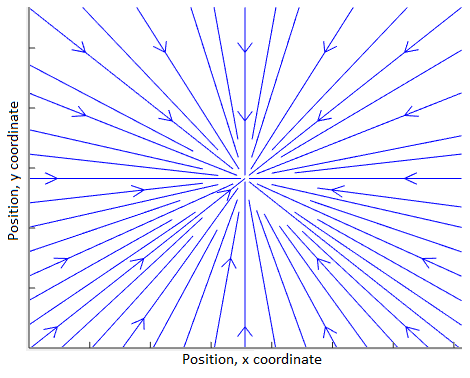
\includegraphics[width=10cm]{img/dynamical_system_empty.png}
\caption{2D representation of the dynamical system.\newline Blue arrows represent the direction to follow for the robot from anywhere in the space, the attractor point is situated in the middle.}
\label{simple_dynamical_system}
\end{figure}

With no corrections, the model will return a straight trajectory from anywhere to the target (see \autoref{simple_dynamical_system}). Also, it's easy to add corrections made by the operator. If a correction is present in the system, all the direction vectors, that initially went through it, should align with the correction (and never cross it). As a result it will curve those direction vectors by applying local little rotations. The rotations will be distributed around the correction by a Gaussian Process Regression, see \autoref{correction_dynamical_system}.

\begin{figure}[H]
\centering
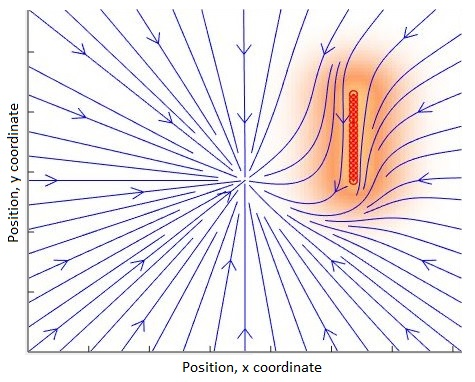
\includegraphics[width=10cm]{img/dynamical_system_1_correction.jpg}
\caption{2D representation of the dynamical system with one correction represented in red and a red gradient showing its influence.}
\label{correction_dynamical_system}
\end{figure}

\subsection{Goals}

After this project, the robot will be able to compute a demonstration and learn about it. The process is done in four steps: first, get the whole demonstration as an input, see \autoref{step1_process}, then numerically isolate the correction, see \autoref{step2_process}, after convert the obtained correction into a continuous function (using cubic splines), see \autoref{step3_process} and finally transmit the correction to the learning algorithm. It will be possible to compute the influence of the correction for any point in the space by applying a Gaussian Process Regression, see \autoref{step4_process}.

\begin{figure}[H]
    \begin{minipage}[b]{0.5\linewidth}
        \centering
        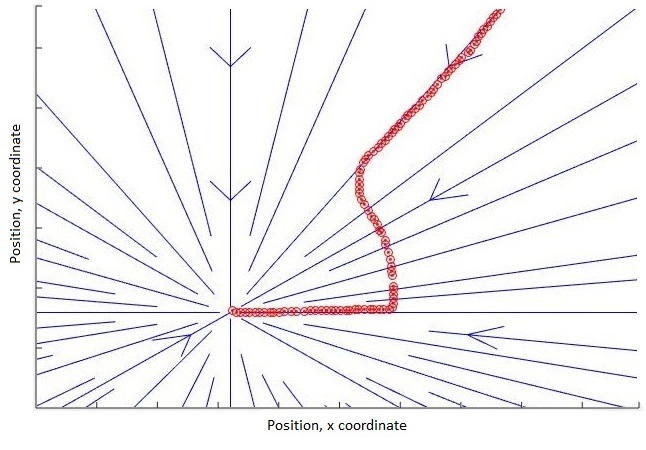
\includegraphics[width=0.95\textwidth]{img/step_1_traj.jpg}
        \caption{\\\hspace{0cm}Step 1: Recording a demonstration.\\\hspace{0cm}Red dots are the demonstration.}
        \label{step1_process}
    \end{minipage}
    \begin{minipage}[b]{0.5\linewidth}
        \centering 
        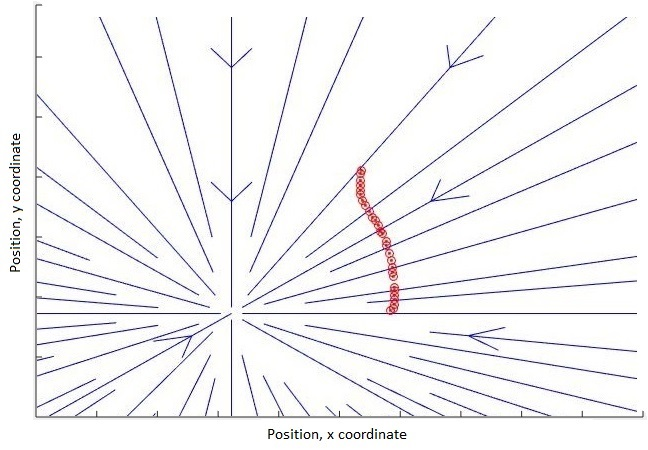
\includegraphics[width=0.95\textwidth]{img/step_2_iso.jpg}
        \caption{\\\hspace{0cm}Step 2: Isolating the correction.\\\hspace{0cm}Red dots only represent the correction.}
        \label{step2_process}
    \end{minipage}\hfill
\end{figure}
\begin{figure}[H]
    \begin{minipage}[b]{0.5\linewidth}
        \centering 
        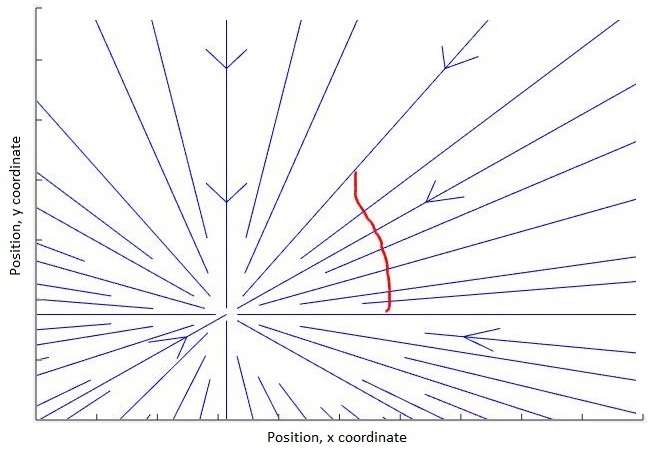
\includegraphics[width=0.95\textwidth]{img/step_3_cont.jpg}
        \caption{\\\hspace{0cm}Step 3: Transforming the correction into a continuous function: spline.\\\hspace{0cm}The red line is the spline.}
        \label{step3_process}
    \end{minipage}
    \begin{minipage}[b]{0.5\linewidth}
        \centering 
        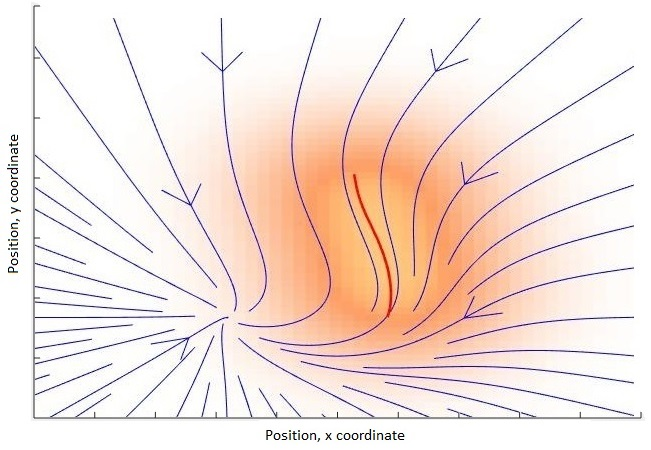
\includegraphics[width=0.95\textwidth]{img/step_4_GPR.jpg}
        \caption{\\\hspace{0cm}Step 4: Computing influence.\\\hspace{0cm}Red gradient show the influence of the correction.}
        \label{step4_process}
    \end{minipage}\hfill
\end{figure}

While using a Gaussian Process Regression in a discrete way to get around corrections, in this special case, some trajectories are still going through the correction instead of aligning to it. To solve this problem, we adapted the GPR for a continuous representation of the correction by using a distance algorithm from a point to a curve.\\